\documentclass{beamer}

%\usepackage[3D]{movie15}
\usepackage{array}
\usepackage{amsmath}
%\usepackage{tikz}
%\usepackage{pgflibraryshapes}  
\usepackage{beamerthemesplit} 
\usetheme{Madrid}
\usepackage[overlay,absolute]{textpos}
\TPGrid[4mm,25mm]{10}{5}


\newcommand{\opal}{\textsc{OPAL }}
\newcommand{\opalcycl}{\textsc{OPAL-cycl }}
\newcommand{\rnb}{radially neighboring bunches }
\newcommand{\sce}{Space charge effects }
\newcommand{\scf}{Space charge force }
\newcommand{\bs}[1]{\mathbf #1}


\AtBeginSection[]
{
  \begin{frame}<beamer>
    \frametitle{Outline}
    \tableofcontents[currentsection,hideothersubsections]
  \end{frame}
}

\title{\opalcycl: A Parallel PIC Code Including Neighboring Bunches Effects in Cyclotron}
%\subtitle{Modeling, Programming and First Result}
\subtitle{Work in Progress}
\author{Jianjun Yang$^1$, Andreas Adelmann$^2$} 
\institute{1. Ph.D Candidate, CIAE \& Tsinghua Univ. \\
  2. AMAS Group, PSI}
\date{22th April, 2008}

\begin{document} 

  \frame{\titlepage} 
  
  \section*{Outline} 

  \frame{\tableofcontents}

  \section{Background \& Motivation} 

  \frame{
    \frametitle{Background}

    \begin{block}{Brief Review} 
      \sce play an important role in high intensity cyclotrons (space charge dominated PSI Injector2).
      Two different types can be distinguished.  
      \begin{itemize}  
      \item \sce of \alert{ single bunch}.\\
	M.M.Gordon, M.Joho, S.Adam, A.Adelmann and P. Bertrand have done very nice work on this. 
      \item \sce of \alert{ \rnb}.\\
	As a pioneer, E.Pozdeyev developed a model in his code CYCO (Ph.D thesis, MSU, 2003) \\
	\alert{$\Rightarrow$} Not self-consistent model \alert{\&} serial code \alert{\&} $\theta$ as independent variable.

      \end{itemize}
    \end{block}
    \begin{columns}
      \begin{column}{6.0cm}
	\includegraphics[width=\linewidth]{figures/Multi-bunch}
      \end{column}
    \end{columns}
  }

  \frame{
    \frametitle{Background}
    \begin{block}{ Turn Separation }
      In an ideal machine, the \alert{''radial gain per turn''} $\Delta R_{n,n+1}$ produced by the increment of energy can be expressed as:\\ 
      
      %      \includegraphics[width=10.0cm]{figures/dRdn.pdf} \\
      \begin{equation*}
	\scriptstyle{\Delta R_{n,n+1}=\left[ \sqrt{1+\frac{2\Delta E_{n,n+1} \left( E_k+E_0\right) + \left( \Delta E_{n,n+1}\right)^2}{2 E_k E_0+E_k{}^2}}\Bigg{/}\left(1+\frac{\Delta E_{n,n+1}}{E_k+E_0}\right)-1 \right]R_n .}
      \end{equation*}


      \center{  $E_0$: rest energy,\\ 
	$E_k$: kinetic energy,\\ 
	$\Delta E_{n,n+1}$ : energy gain in one turn,\\
	$R_n$: average radius of $n$th turn.\\
      }
    \end{block}
    \begin{block}{}
      If $\Delta E_{n,n+1}$ keeps constant,  $E_k \nearrow $ \ $\Rightarrow$ \  $\Delta R_{n,n+1} \searrow $ 
    \end{block} 

  }


  %\frame{
  % \frametitle{ Turn Seperation }
  % \begin{block}{}
   % In extraction point, the ''radial gain per turn'' of reference orbit produced by the increment of energy can be expressed as:
  % \begin{equation}
  %   \frac{dR}{dn} = R\cdot\frac{E_G}{E}\cdot\frac{\gamma}{\gamma+1}\cdot\frac{1}{\nu^{2}_{r}}
  % \end{equation}
  % $R$: average radius of orbit,\\
  % $E$: kinetic energy,\\ 
  % $E_G$: energy gain per turn,\\
  % $\gamma$: relativistic factor,\\
  % $\nu_r$: radial betatran osillation frequency.   
  % \end{block}
  %}

  \frame{
    \frametitle{Motivation: Upgrade Project of PSI Cyclotron Facility}
    \begin{columns}
      \begin{column}{6.0cm}
	\begin{block}{590MeV Ring}
          \begin{itemize}
          \item Beam Current/Power:\\ 
	    \alert{2mA/1.2MW} $\Rightarrow$ \alert{3mA/1.8MW}\\
	    The \alert {highest current} cyclotron in the world.
	  \item Turns number \\
	    \alert{~200} $\Rightarrow$ less than \alert{160}.
	  \item After upgrade, turn seperation better.  
	  \end{itemize}
	\end{block}
      \end{column}

      \begin{column}{6.0cm}
	\includegraphics[width=\linewidth]{figures/ringcyc}
      \end{column}
    \end{columns}
    \begin{block}{}
      After upgrade, without deliberately added field for extraction purpose, at extraction point,
      \center $\Delta R_{n,n+1}=5.7$mm. 
    \end{block}
  }

  \frame{
    \frametitle{Motivation: Compact Cyclotron under Building in CIAE}
    \begin{columns}
      \begin{column}{6.0cm}
	\begin{block}{100MeV $H^-$ CYCIAE-100}
          \begin{itemize}
          \item Designed beam current \alert{0.2mA}, future \alert{0.5mA} .
	  \item Turns number is about \alert{~500}.
	  \item Energy gain per turn is \alert{0.2MeV}.
	  \item Multi-turn extraction by striper at radius of \alert{1.9m}.
	  \item Turn separation far smaller than beam size at outer Radius, multi-bunches will \alert{overlap together}. 
	  \end{itemize}
	\end{block}
      \end{column}

      \begin{column}{6.0cm}
	\includegraphics[width=\linewidth]{figures/cyciae100.png}
      \end{column}
    \end{columns}
    \begin{block}{}
      At extraction point, 
      \center $\Delta R_{n,n+1}=1.5$mm. 
    \end{block}
  }

  \section{Mathematical model and Algorithm}
%  \subsection{some basic knowledge}
  \frame{
    \frametitle{Basic Formula}

    \begin{block}{Particle Motion Equation}
      Common equations of motion of single charged particle in electromagnetic field.
      \footnotesize
      \begin{equation*}
	\dot{\bs{p}} = \bs{F}(\bs{v},\bs{x},t) = q\;(\bs{v} \times \bs{B} + \bs{E})
      \end{equation*}
      \begin{equation*}
	\bs{E} = \bs{E_{ext}}+\bs{E_{sc}}
      \end{equation*}
      \begin{equation*}
	\bs{B} = \bs{B_{ext}}+\bs{B_{sc}}
      \end{equation*}
    \end{block}

    \begin{block}{}
      the evolution of beam's distribution function $ f(\bs {x},\bs{v},t)$ can be expressed by collisonless Vlasov-Maxwell Equations:    
      \footnotesize
      \begin{equation*}
	\frac{df}{dt}=\partial_t f + \bs{v}\cdot \nabla_x f +\frac{q}{m}(\bs{E}+ \bs{v}\times\bs{B})\cdot \nabla_v f  =  0 .
      \end{equation*}
      %\begin{displaymath}
      %\begin{array}{rccccc}
	%  c^{-2} \partial_t\bs{E} &-& \nabla\times\bs{B} & = & -\mu_0 & \bs{J}      \\
	 % \partial_t\bs{B} &+& \nabla\times\bs{E} & = &     0  &                  \\
      	 % & & \nabla \cdot \bs{E}         & = & \epsilon_0^{-1}&\rho \\
	 % & & \nabla \cdot \bs{B}         & = &    0    &   \\ \\
       % \end{array}
      %\end{displaymath}

    \end{block}

  }

  \begin{frame}
    \frametitle{3D Parallel Poisson equation Solver using PIC/FFT}  
    
    \begin{block}{}
     The external fields are given, space charge field can be obtain by solving 
     Poisson equation using PIC (Particle-In-Cell) methods.
    \end{block}

    \begin{block} {Solve Poisson equation on discrete domain}  
      In PIC/FFT, a 3D rectangle grid which contains all particles is built(following quantities with superscript of $D$ means on grid).
      
      The solution of the discretized Poisson equation with $\vec{k}=(l,n,m,)$
      \begin{equation*}\label{eq:DiscretizedPoisson}
	\nabla^{2} \phi^D(\vec{k}) = - \frac{\rho^D(\vec{k})}{\epsilon_0}, \vec{k} \in \Omega^D.
      \end{equation*}
      
      $\phi^D$ is given by convolution with the appropriate discretized Green's function $G_D$: 
      \begin{equation*}
	\phi^D = \rho^D * G^D.
      \end{equation*}
    \end{block}
%     \begin{center}                                                                                                                     
%      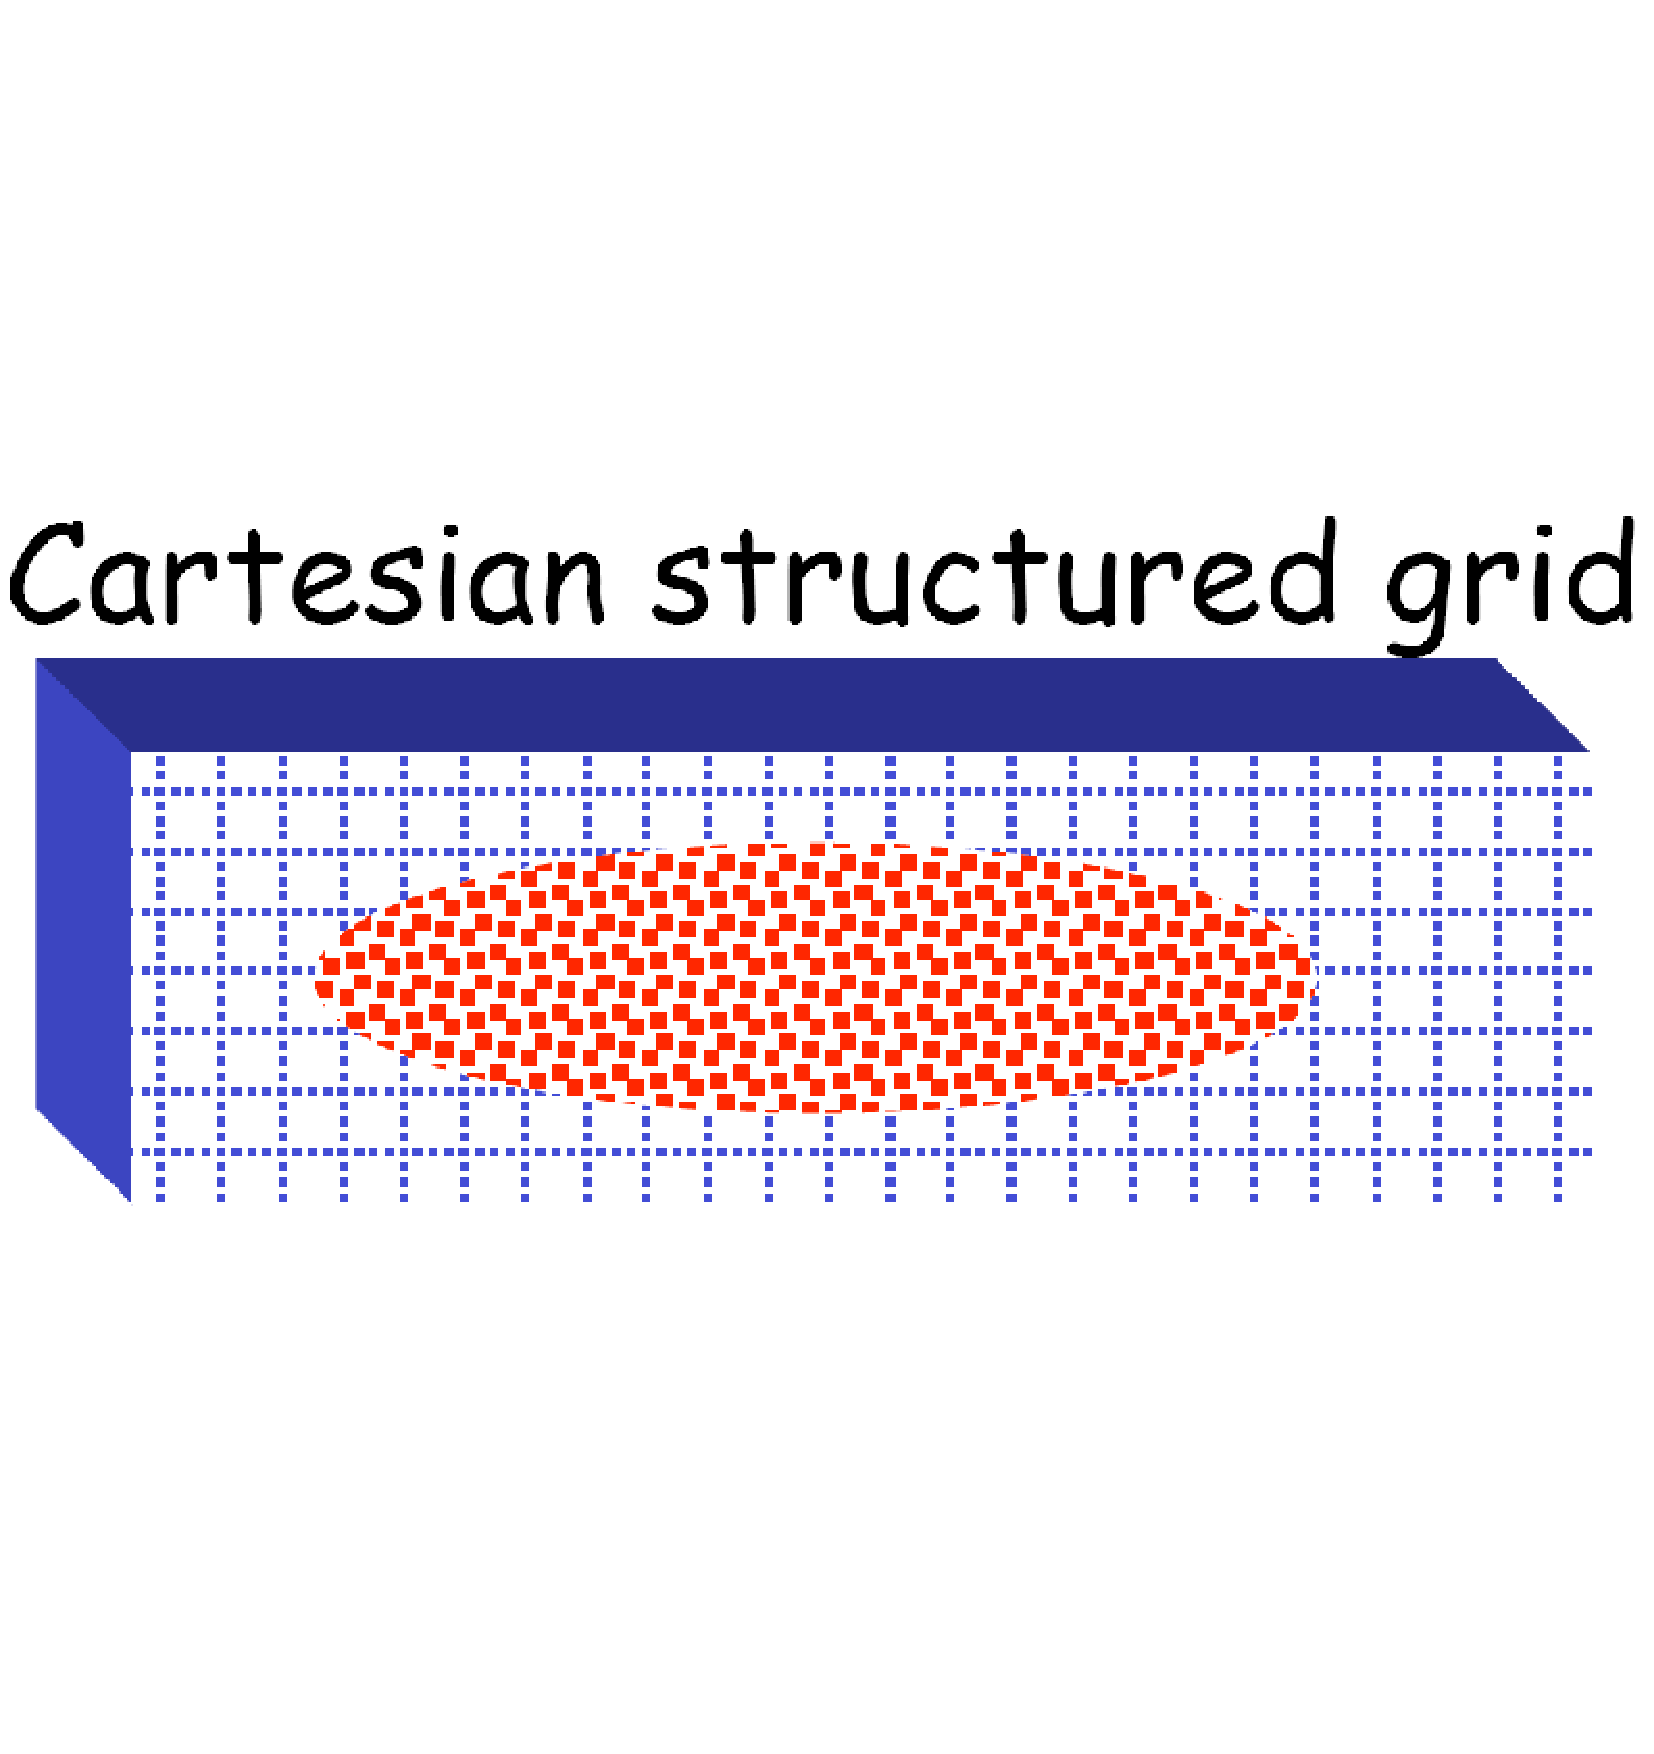
\includegraphics[width=5.0cm]{figures/Grid}                                                                   \end{center}  
  \end{frame}

  \begin{frame}
    \frametitle{3D Parallel Poisson Solver using PIC/FFT}  
    \begin{center}
      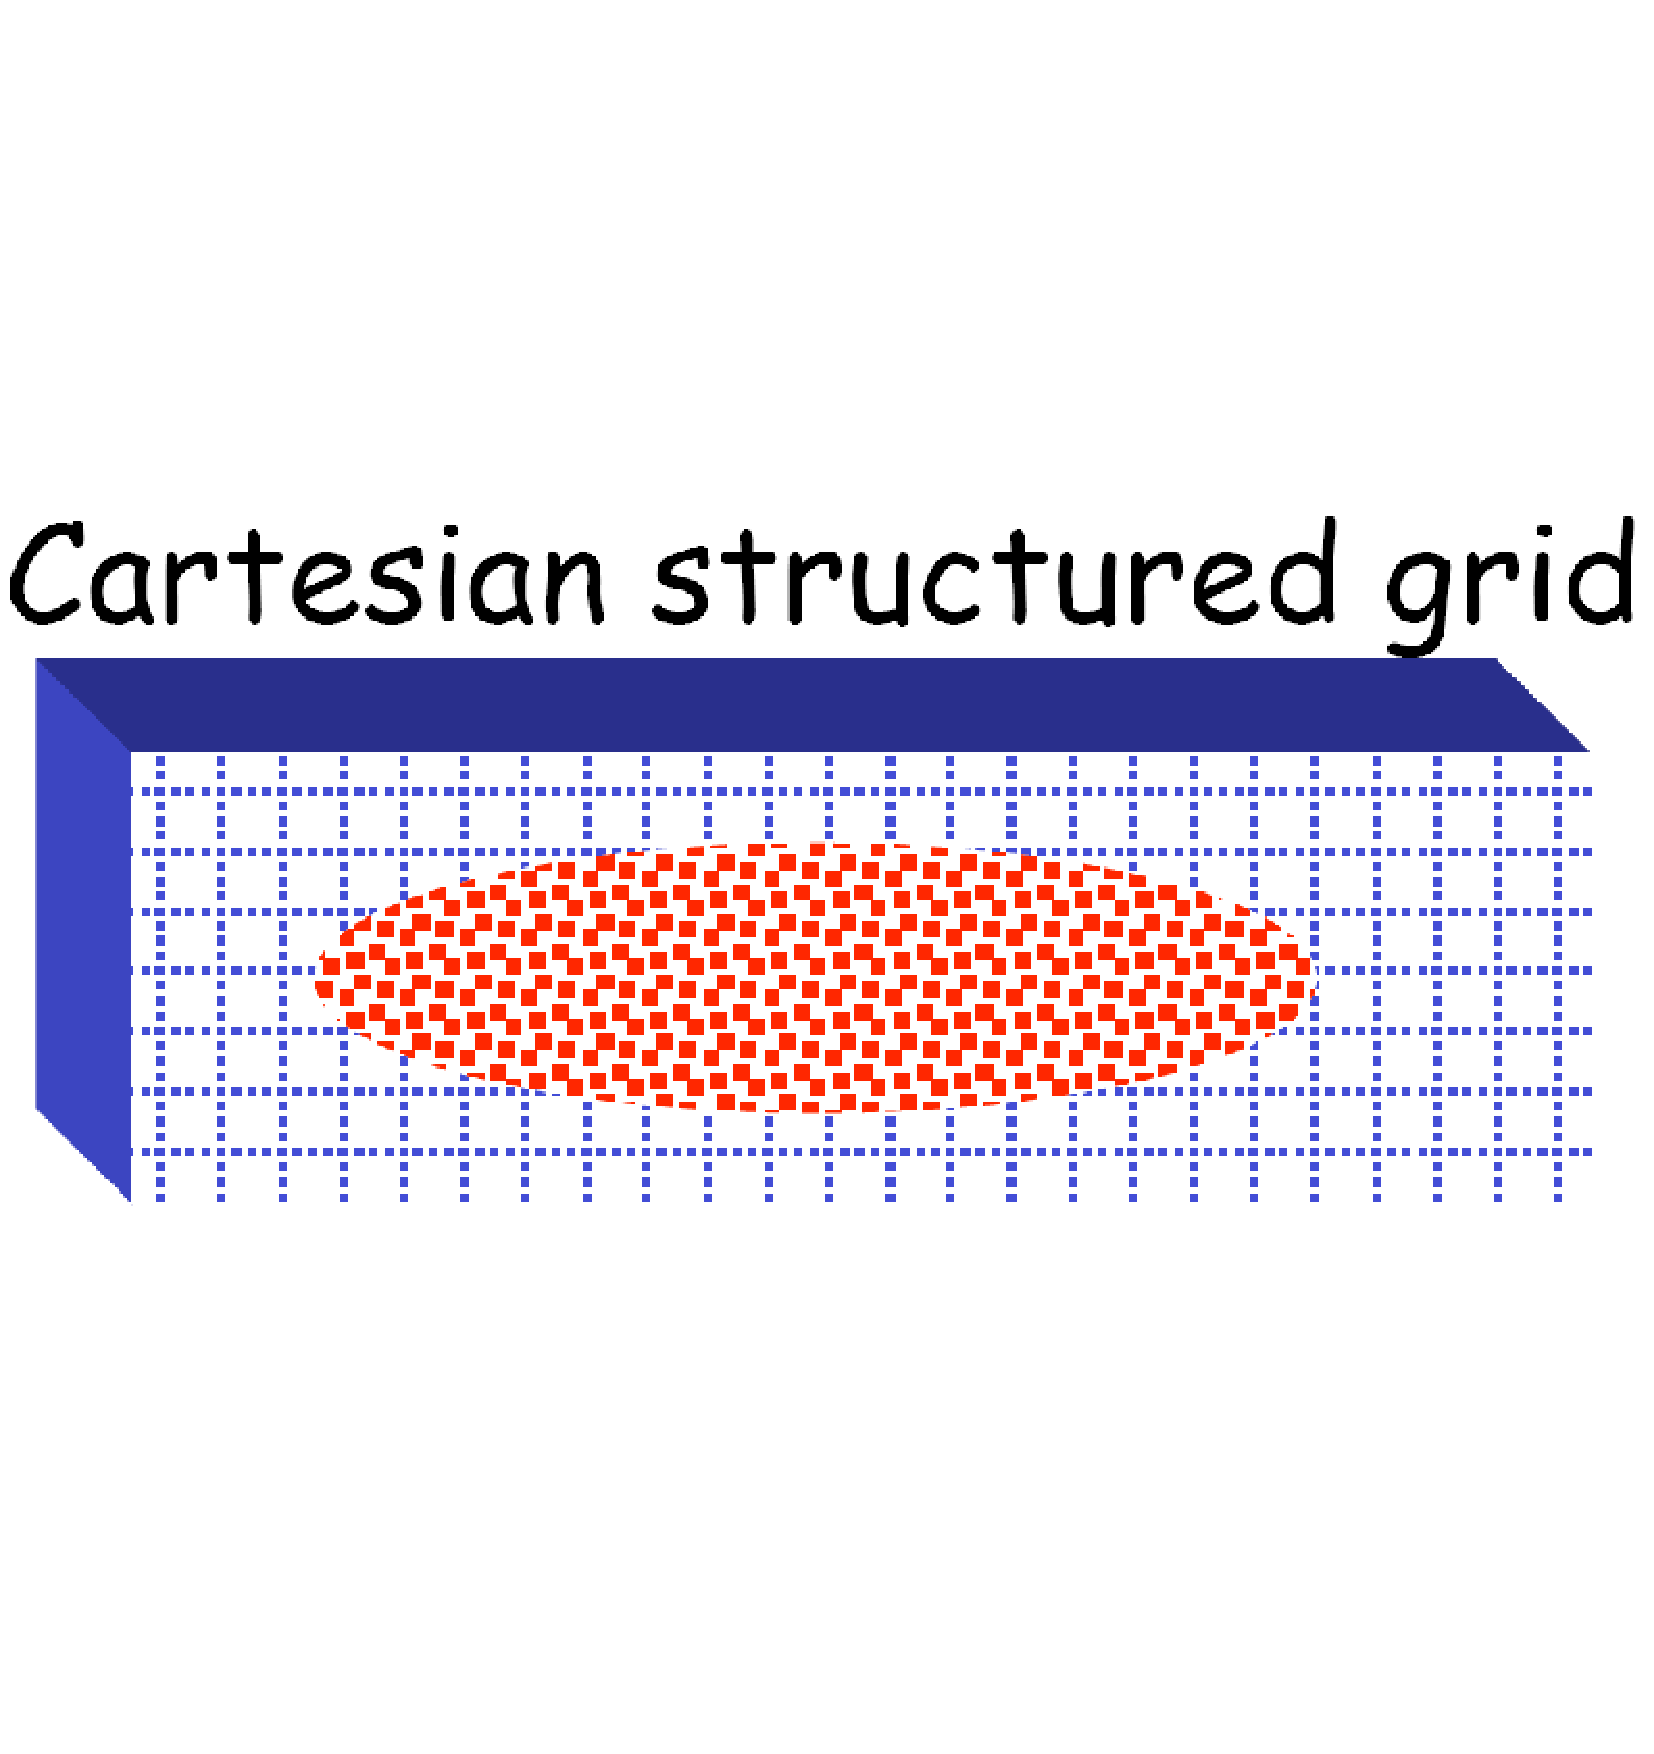
\includegraphics[width=5.0cm]{figures/Grid}
    \end{center}
    \begin{block}{Basic Process of the Poisson Solver}
      \begin{tabbing}
	\quad $\triangleright$ Assign all particles charges $q_i$ to nearby mesh points to obtain $\rho^D$\\
	\pause
	\quad $\triangleright$ Lorentz transform to obtain $\rho^D$ in beam rest frame $\bs{S_{beam}}$.\\
	\pause
	\quad $\triangleright$ Use FFT on $\rho^D$ and $G^D$ to obtain $\widehat{\rho}^D$ and $\widehat{G}^D$ \\
	\pause
	\quad $\triangleright$ Determine $\widehat{\phi}^D$ on the grid using $\widehat{\phi}^D = \widehat{\rho}^D \cdot \widehat{G}^D$  \\
	\pause
	\quad $\triangleright$ Use inverse FFT on $\widehat{\phi }^D$ to obtain $\phi^D$ \\
	\pause
	\quad $\triangleright$ Compute $\bs{E}^D= -\nabla \phi^D$\\
	\pause
	\quad $\triangleright$ Interpolate $\bs{E}$ at particle positions $\bs{x}$ from $\bs{E}^D$  \\
	\pause
	\quad $\triangleright$ Lorentz back transform to obtain $\bs{E_{sc}}$ and $\bs{B_{sc}}$ in laboratory frame $\bs{S_{lab}}$.\\ 
      \end{tabbing}
    \end{block}
    
  \end{frame}


  %\frame{
  % \frametitle{Some Comments}
  % \begin{block}{Comments on PIC/FFT}
  %  \begin{tabbing}
  %   \quad $\triangleright$ has high efficency for large scale particles compare with P-P method;\\
  %  because of its loose dependency on particles number.\\
  %  \quad $\triangleright$ can gain high presicion in accelerator simulation; \\
  %  where particles are basically propergate in the same direction.\\ 
  %  \quad $\triangleright$ FFT Algrothm is fit for parallelization.\\ 
  % \end{tabbing}
  %\end{block}
  %}

  \frame{
    \frametitle{3D Parallel Poisson Solver using PIC/FFT}  
    \begin{block}{Specialization in Cyclotron}
      \begin{itemize}
	\item The orientation of laboratory frame $\bs{S_{lab}}$ changes from time to time.\\ %cause the reference orbit is a spiral outerwards curve.
	\item  For multi-bunch simulation, the energy span is huge, so particles are divided into different \alert{energy bins}. 
	For each bin, apply Lorentz transformation and calculate field. 
	%\quad $\triangleright$  Strong coupling between longitudinal and transversal direction.\\ % which causes the motion of particles in the bunch more complcated.
	%\center $\Rightarrow$ \alert {Azimuthal energy spread and phase width can increase radial size sufficiently!}
      \end{itemize}
    \end{block}

    \begin{columns}
      \begin{column}{8.0cm}
	\includegraphics[width=\linewidth]{figures/Multi-bunch}
      \end{column}
    \end{columns}
  }

  \section{Implementation of \opalcycl}

  \frame{
    \frametitle{ Implementation of \opalcycl}
    \begin{block}{Characteristics of \opalcycl}   
      \begin{itemize}
      \item Based on OPAL framework (IPPL, CLASSIC, H5Part, HDF5)
      \item Store intermediate phase space data in hdf5 format
      \item Read in measured field map of median plane
      \item Treat electric field of cavity as a $\delta$ function with correction of transit effects
      \item Use 4th-order RK as integrator
      \item Use time as independent variable
      \item Track in global cartesian coordinates
      \item Has three working modes: 
	\begin{itemize}
	\item Single particle tracking mode.
	\item Tune calculation mode.
	\item Multi-bunches tracking mode (single bunch \& multi-bunches) 
	\end{itemize}
      \end{itemize}
    \end{block}
  }

  \frame{
    \frametitle{ Implementation of \opalcycl}
    \begin{block}{ Implement neighboring bunches effects in electrostatic approximation}
      \begin{itemize}
      \item When $\Delta R \le M \sigma_{x,y}$ , the execution will transfers from \alert {single bunch mode} 
	to \alert{multi-bunch mode} automatically, namely, inject new bunches consecutively after each revolution period.
      \item Integrate particles in all the bunches simutaniously.
      \item For each time step, calculate space charge field for each energy bin using PIC/FFT, then add contribution of all bins 
	together.
      \item Reset energy bin when the bunches' energy span overlap together.  	
      \end{itemize}
    \end{block}
     \begin{block}{}
       \center \alert{Fully self-consistent model of dealing with \rnb effects in time domain!}
    \end{block}
  }

  \section{First results on Ring and Injector2}
  
  \subsection{Single particle track result}

  \frame{
    \frametitle{Single particle track result}
    \begin{block}{Reference Orbit of Ring}
      Before upgrade, set $V_{main} = 0.735MV,V_{flat top} = 11.2\%V_{main}$,\alert{206} turns \\ 
      After  upgrade, set $V_{main} = 0.900MV,V_{flat top} = 11.2\%V_{main}$,\alert{168} turns  
    \end{block}
    \begin{columns}
      \begin{column}{7.0cm}
	\includegraphics[width=\linewidth]{figures/AEO-Ring.png}         
      \end{column}
      \begin{column}{4.0cm}
	\includegraphics[width=\linewidth]{figures/Extraction_Ring.png}         
      \end{column}
    \end{columns}
  }

  \frame{
    \frametitle{Single particle track result}
    \begin{columns}
      \begin{column}{7.0cm}
	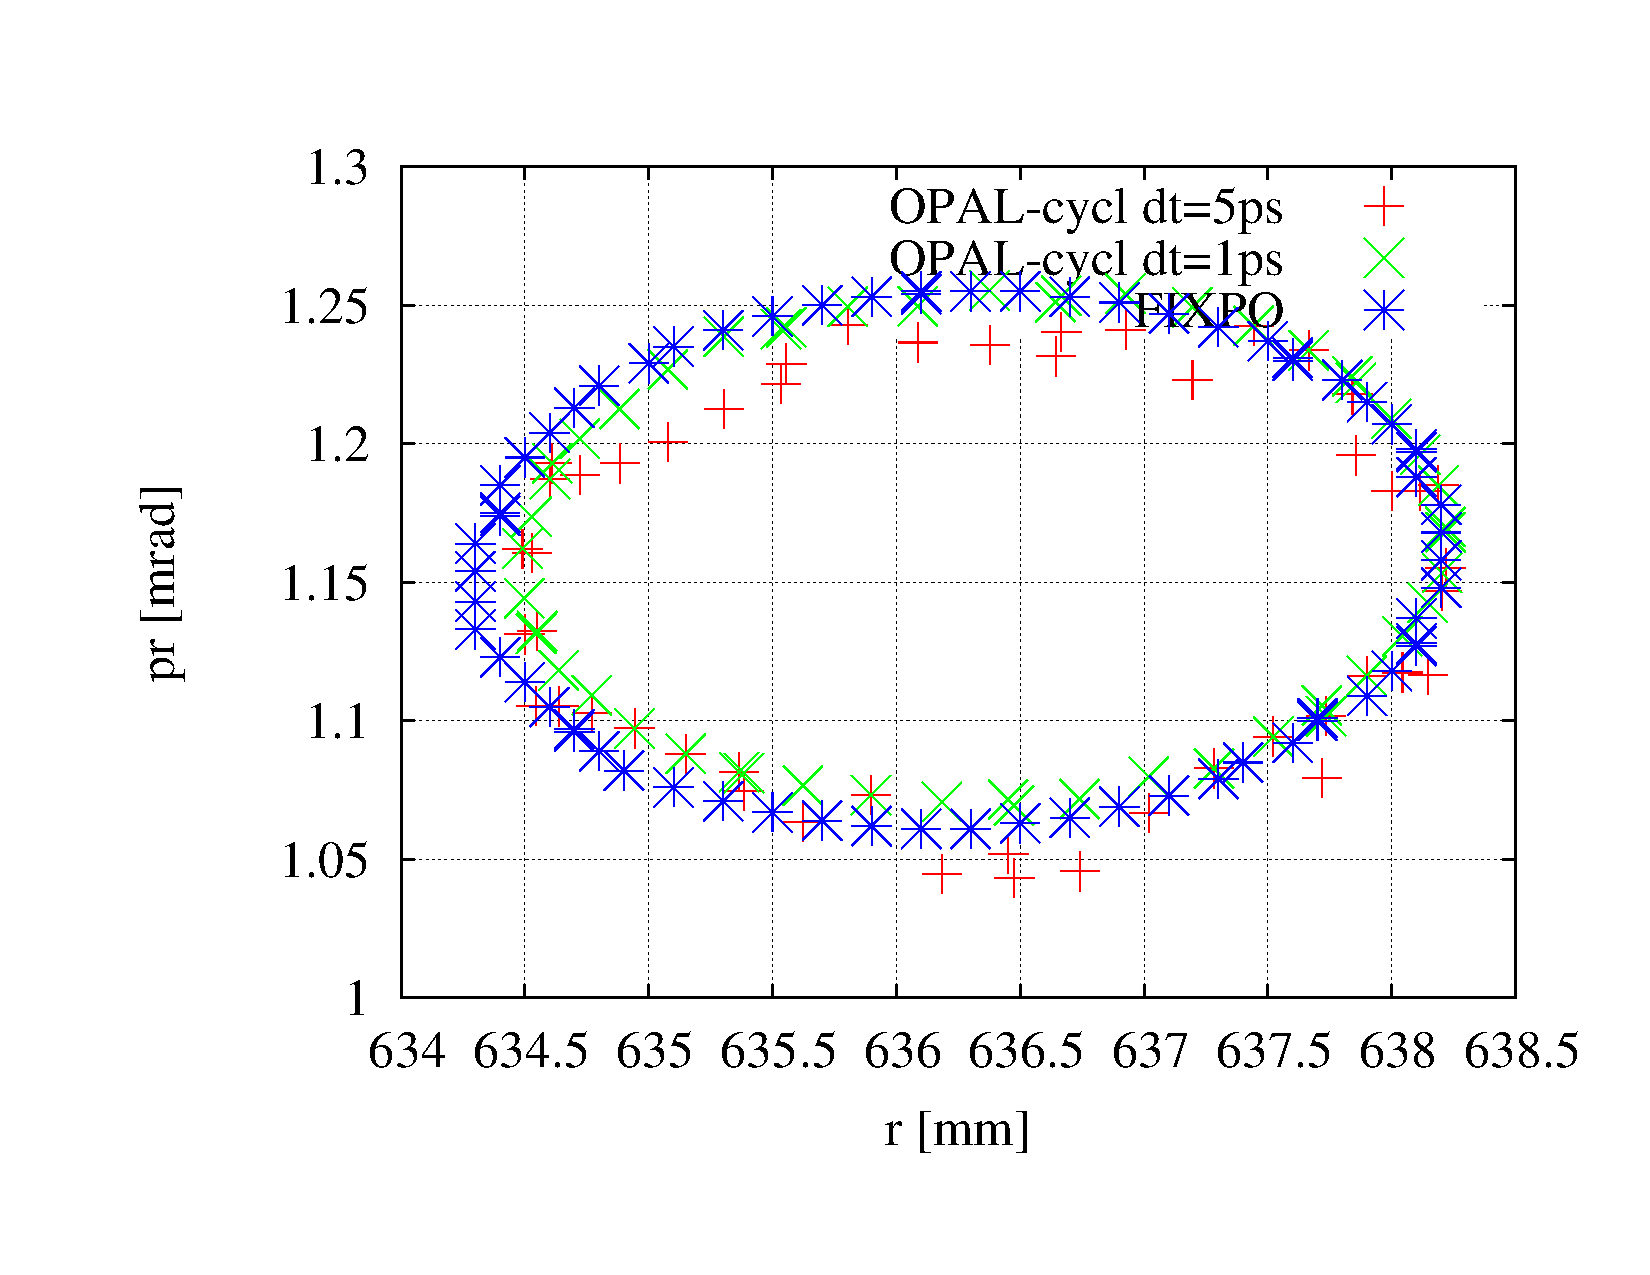
\includegraphics[width=\linewidth]{figures/RadialEigen_Inj2}         
      \end{column}
    \end{columns}
    \begin{block}{Eigen ellipse of Inj.2 @ 2MeV}
	  Radial eigen ellipse agree with FIXPO code very well !      
    \end{block}
  }

  \subsection{Tune calculation result}

  \frame{
    \frametitle{Tune calculation result}   
    \begin{columns}
      \begin{column}{6.5cm}
	\center {PSI Ring}
	\includegraphics[width=\linewidth]{figures/nurnuz_Ring}         
      \end{column}
      \begin{column}{6.5cm}
	\center {PSI Injector2}
	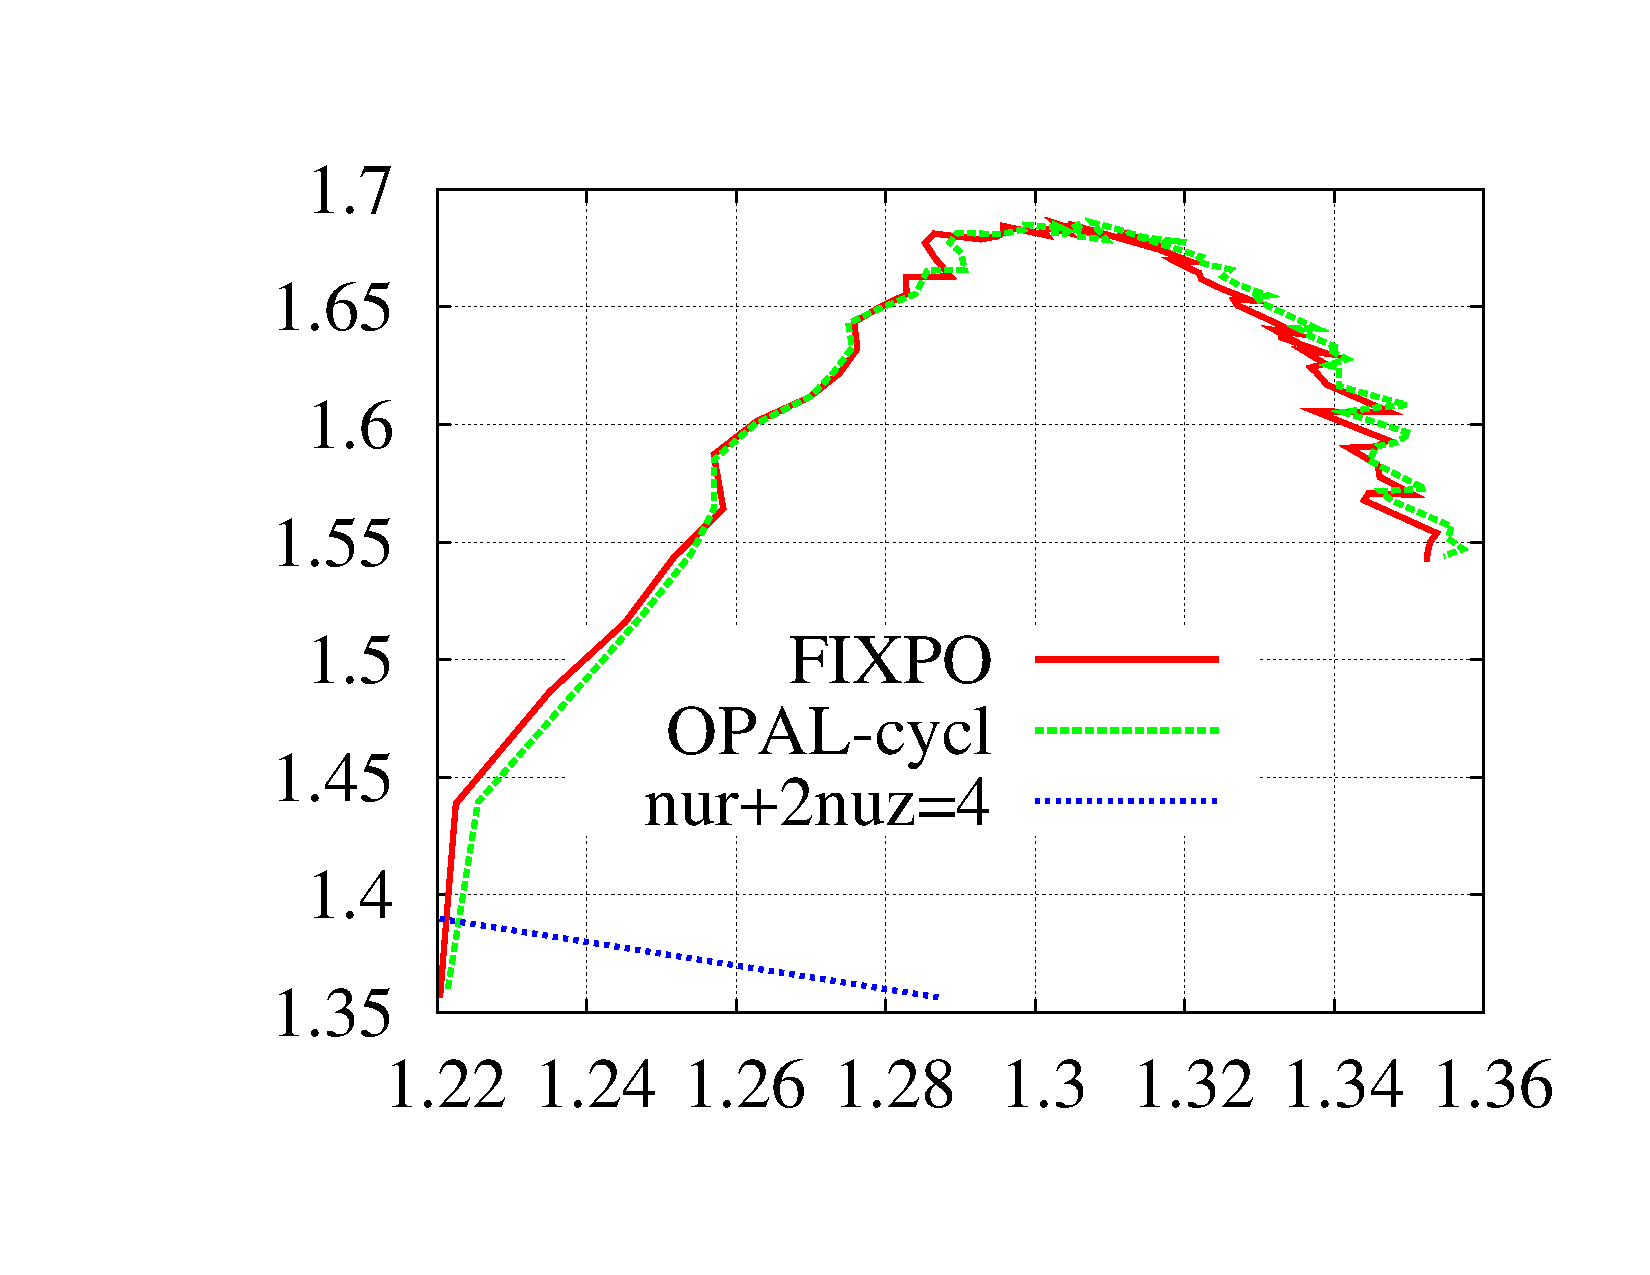
\includegraphics[width=\linewidth]{figures/nurnuz_Inj2}         
      \end{column}
    \end{columns}

    \begin{block}{Tune diagram}
      The calculation results agree with FIXPO code very well !      
    \end{block}
  }

  \subsection{\opalcycl Scaling }
  
  \begin{frame} 
    \frametitle{Test for parallel Scalability}
{\opalcycl Scaling on Cray XT3 Cluster at CSCS}
    \begin{columns}
      \begin{column}{4.cm}
	\scriptsize
	\begin{block}{Production Run Setup}
          \begin{itemize}
          \item $10^6$ particles 
          \item 3D FFT on a $64^3$ grid
	  \item 2D domain decomposition 
	  \item track 200 time steps
          \item Gaussian distribution
	  \item Dump data into single HDF5 file
          \end{itemize}
	\end{block}
	
	\begin{block}{Observations}
          \begin{itemize}
          \item The code scales well
	  \item Good load-balancing
	  \item 128 processors is best choice for this job.
          \end{itemize}
	\end{block}
      \end{column}
      \begin{column}{7.0cm}
	\includegraphics[width=\linewidth]{figures/Timing64mesh}         
      \end{column}
    \end{columns}
  \end{frame}


  \subsection{Single bunch and multi-bunch result}
  
  \frame{
    \frametitle{Animation of Single Bunches and Multi-Bunches}
    
    \begin{block}{Movies show}
      \center {Single Bunch Run }
      \center {3 Bunches Run }
    \end{block}

  }

  \frame{
    \frametitle{Multi-Bunches Test in Ring}
    \begin{columns}
      \begin{column}{6.0cm}
	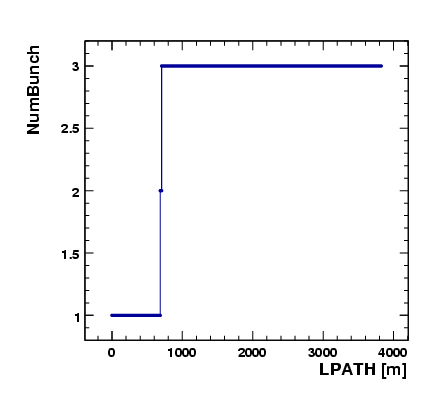
\includegraphics[width=\linewidth]{figures/Ring3Bunch-NumBunch-LPATH.png}
      \end{column}
      \begin{column}{6.0cm}
	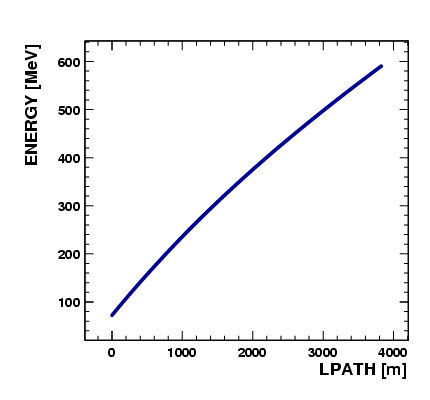
\includegraphics[width=\linewidth]{figures/Ring3Bunch-ENERGY-LPATH.png}
      \end{column}
    \end{columns}
  }

  \frame{
    \frametitle{Multi-Bunches Test in Ring}

    \begin{block}{}
      \center {Single Bunch Run}
    \end{block}

    \begin{columns}
      \begin{column}{4.0cm}
	\center {40th turn}
	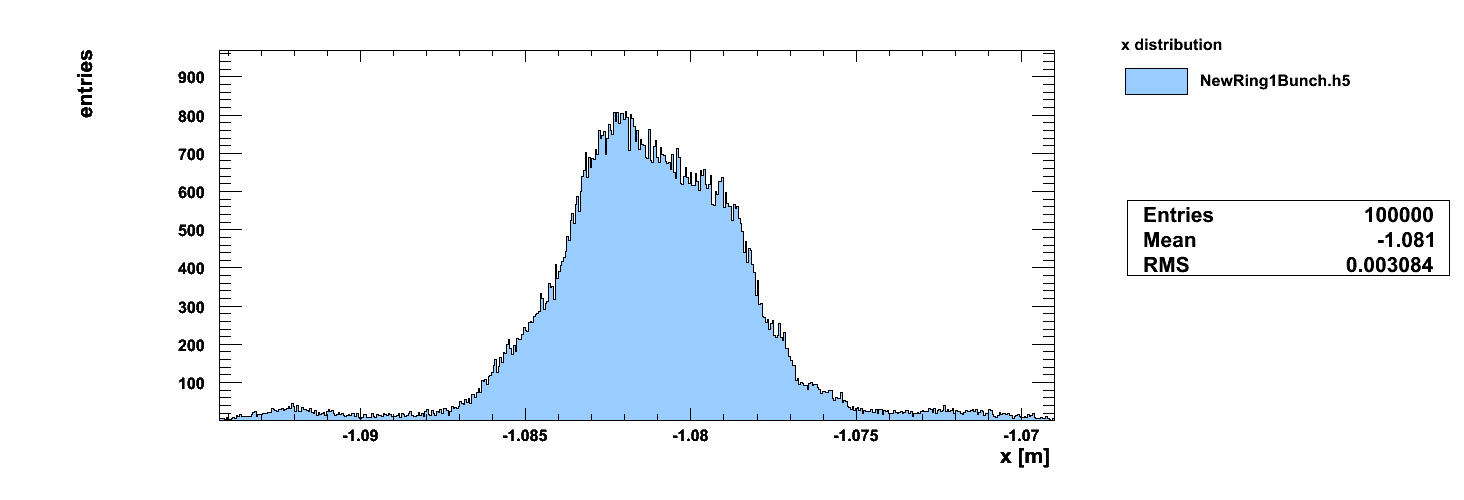
\includegraphics[width=\linewidth]{figures/NewRing1Bunch-x-step-2387.png}         
      \end{column}
      \begin{column}{4.0cm}
	\center {41th turn}
	\includegraphics[width=\linewidth]{figures/NewRing1Bunch-x-step-2446.png}         
      \end{column}
      \begin{column}{4.0cm}
	\center {42th turn}
	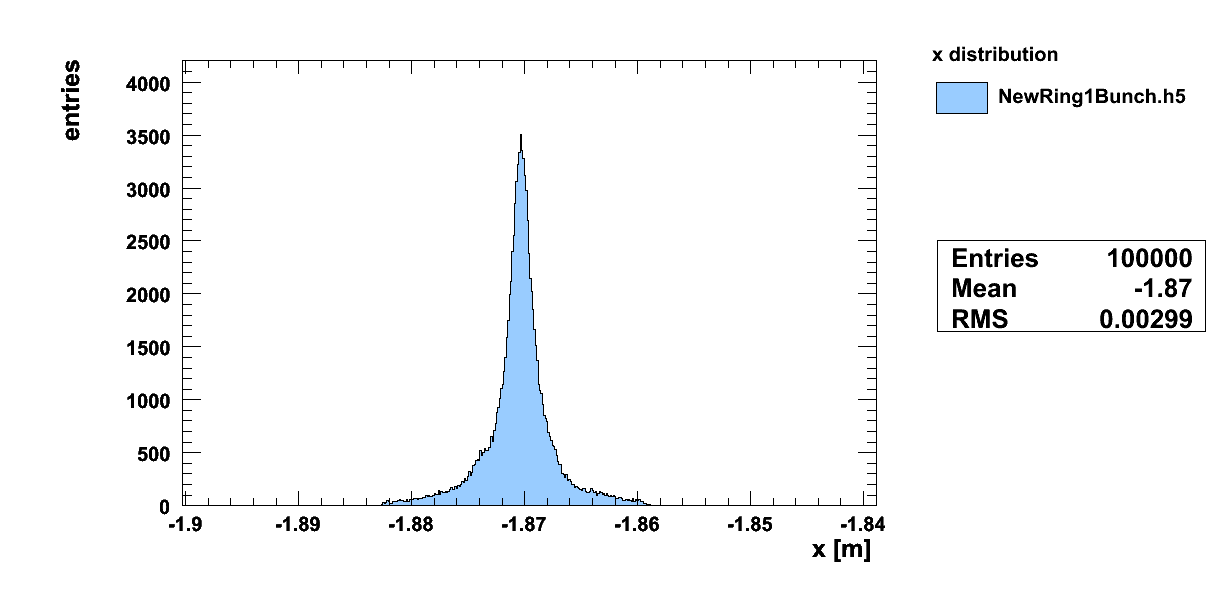
\includegraphics[width=\linewidth]{figures/NewRing1Bunch-x-step-2508.png}         
      \end{column}
    \end{columns}

    \begin{block}{}
      \center {3 Bunches Run}
    \end{block}
    \begin{columns}
      \begin{column}{4.0cm}
	% \center {SingleBunch}
	\center {40th turn}
	\includegraphics[width=\linewidth]{figures/Ring3Bunch-x-step-2388.png}         
      \end{column}
      \begin{column}{4.0cm}
	\center {41th turn}
	%\center {Single Bunch}
	\includegraphics[width=\linewidth]{figures/Ring3Bunch-x-step-2447.png}         
      \end{column}
      \begin{column}{4.0cm}
	\center {42th turn}
	% \center {PSI Injector2}
	\includegraphics[width=\linewidth]{figures/Ring3Bunch-x-step-2509.png}         
      \end{column}
    \end{columns}
  }

  \frame{
    \frametitle{Outlook}
    \begin{block}{Future plan}
      \begin{itemize}
      \item Study in detail on beam dynamics issues of PSI Ring and CYCIAE-100 machine to do some substantial contribution.
      \item Add Radial and vertical collimator.
      \item Include high order expansion of magnetic field, RF magnetic field.

      \end{itemize}
    \end{block}
  }

  \section{Acknowledgments}
  \frame{
    \frametitle{Acknowledgments}
    \begin{block}{Many Thanks To :}
      \center{
	T.J. Zhang\\
	M. Humbel \\
	Ch. Kraus \\ 
	W. Joho \\
	AMAS Group Members \\   
      }
    \end{block}
  }

    \end{document}
